\section{Architettura}

L'architettura del prodotto è suddivisa in:
	\begin{itemize}
	  	\item \textbf{gateway};
	  	\item \textbf{piattaforma Apache Kafka};
	  	\item \textbf{data collector};
	  	\item \textbf{database PostgreSQL e Timeseries};
	  	\item \textbf{API REST};
	  	\item \textbf{bot Telegram};
	  	\item \textbf{web application}.    
	\end{itemize} 

	\begin{figure}[H]
		\centering
		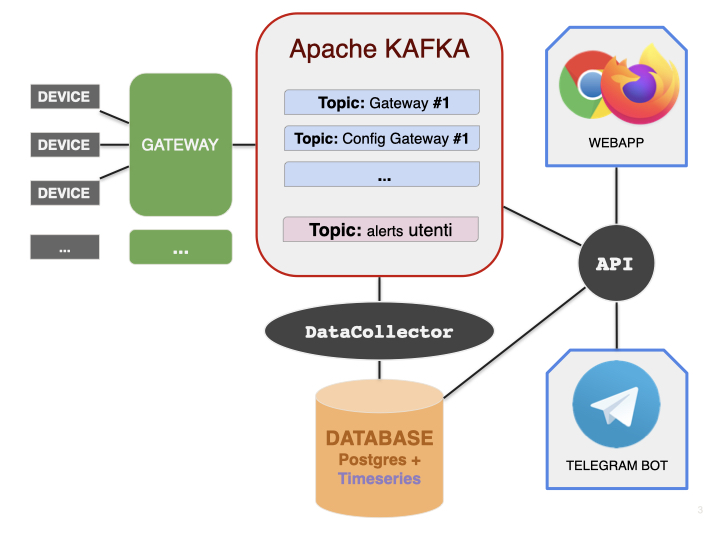
\includegraphics[scale=0.600]{res/images/architetturaGenerale.jpeg}
		\caption{Schema riassuntivo dell'architettura generale del prodotto}
	\end{figure}
	
	\subsection{Interazione tra i componenti}
	Il gateway interagisce con Kafka scrivendo, su un apposito topic di quest'ultimo, i dati che riceve dai sensori ad esso connessi, tramite un producer, in formato \glock{JSON}.
	\newline
	Esso è connesso anche a un secondo topic, tramite un consumer, in modo da permettere agli utenti della web app, che ne abbiano i permessi, di impostarne una diversa configurazione.
	\newline
	La componente data collector si interpone tra i client (web app e bot Telegram), Kafka e i database, con lo scopo di tradurre i dati \glock{JSON} salvati nel topic, a cui è connesso tramite un producer, in record per le tabelle del Timeseries db.
	\newline
	Le \glock{API}, che contengono la business logic, si interpongono tra i client, ovvero bot Telegram e web app, Kafka e ai database.
	\newline
	La connessione API-client si attua tramite richieste e risposte HTTP e il passaggio dei dati tra queste componenti avviene tramite oggetti in formato JSON; la comunicazione API-Kafka, invece, avviene tramite un producer collegato ad un topic, per permettere agli utenti che ne abbiano i permessi, di inviare nuove configurazioni ai gateway.
	\newline
	Infine la connessione tra API e Database avviene tramite il framework JPA, fornito da Spring.  
	
\yetAnotherSectionNamed{gateway}
\yetAnotherSectionNamed{kafka}
\yetAnotherSectionNamed{dataCollector}
\yetAnotherSectionNamed{database}
\yetAnotherSectionNamed{api}
\yetAnotherSectionNamed{telegram}
\yetAnotherSectionNamed{webApp}